
\documentclass[12pt]{article}

% Layout.
\usepackage[top=1in, bottom=0.75in, left=1in, right=1in, headheight=1in, headsep=6pt]{geometry}

% Fonts.
\usepackage{mathptmx}
\usepackage[scaled=0.86]{helvet}
\renewcommand{\emph}[1]{\textsf{\textbf{#1}}}

% TiKZ.
\usepackage{tikz, pgfplots,mathrsfs}
\usetikzlibrary{calc}
\pgfplotsset{compat = newest}
 
\pgfplotsset{my style/.append style={axis x line=middle, axis y line=
middle, xlabel={$x$}, ylabel={$y$}, axis equal
}}

% Misc packages.
\usepackage{amsmath,amssymb,latexsym}
\usepackage{graphicx}
\usepackage{array}
\usepackage{xcolor}
\usepackage{multicol}

% Commands to set various header/footer components.
\makeatletter
\def\doctitle#1{\gdef\@doctitle{#1}}
\doctitle{Use {\tt\textbackslash doctitle\{MY LABEL\}}.}
\def\docdate#1{\gdef\@docdate{#1}}
\docdate{Use {\tt\textbackslash docdate\{MY DATE\}}.}
\def\doccourse#1{\gdef\@doccourse{#1}}
\let\@doccourse\@empty
\def\docscoring#1{\gdef\@docscoring{#1}}
\let\@docscoring\@empty
\def\docversion#1{\gdef\@docversion{#1}}
\let\@docversion\@empty
\makeatother

% Headers and footers layout.
\makeatletter
\usepackage{fancyhdr}
\pagestyle{fancy}
\fancyhf{} % Clears all headers/footers.
\lhead{\baselineskip 30pt
%\emph{\@doctitle\hfill\@docdate}
\emph{\@docdate\hfill\@doctitle}
\ifnum \value{page} > 1\relax\else\\
\emph{Name: \rule{3.5in}{1pt}\hfill \@docscoring}\fi}
\rfoot{\emph{\@docversion}}
\lfoot{\emph{\@doccourse}}
\cfoot{\emph{\thepage}}
\renewcommand{\headrulewidth}{0pt}%
\makeatother

% Paragraph spacing
\parindent 0pt
\parskip 6pt plus 1pt

% A problem is a section-like command. Use \problem{5} to
% start a problem worth 5 points.
\newcounter{probcount}
\newcounter{subprobcount}
\setcounter{probcount}{0}
\newcommand{\problem}[1]{%
\par
\addvspace{4pt}%
\setcounter{subprobcount}{0}%
\stepcounter{probcount}%
\makebox[0pt][r]{\emph{\arabic{probcount}.}\hskip1ex}\emph{[#1 points]}\hskip1ex}
\newcommand{\thesubproblem}{\emph{\alph{subprobcount}.}}

% Subproblems are an enumerate-like environment with a consistent
% numbering scheme. 
% Use \begin{subproblems}\item...\item...\end{subproblems}
\newenvironment{subproblems}{%
\begin{enumerate}%
\setcounter{enumi}{\value{subprobcount}}%
\renewcommand{\theenumi}{\emph{\alph{enumi}}}}%
{\setcounter{subprobcount}{\value{enumi}}\end{enumerate}}

% Blanks for answers in normal and math mode.
\newcommand{\blank}[1]{\rule{#1}{0.75pt}}
\newcommand{\mblank}[1]{\underline{\hspace{#1}}}
\def\emptybox(#1,#2){\framebox{\parbox[c][#2]{#1}{\rule{0pt}{0pt}}}}

% Misc.
\renewcommand{\d}{\displaystyle}
\newcommand{\ds}{\displaystyle}
\def\bc{\begin{center}}
\def\ec{\end{center}}
\def\be{\begin{enumerate}}
\def\ee{\end{enumerate}}


\doctitle{Math 251: Quiz 10}
\docdate{April 14, 2022}
\doccourse{UAF Calculus I}
\docversion{v-1}
\docscoring{\blank{0.8in} / 25}
\begin{document}
%\textbf{Please circle your instructor's name:} \hfill Leah Berman  \hfill   Jill Faudree\\

There are 25 points possible on this quiz. No aids (book, calculator, etc.)
are permitted.  {\bf Show all work for full credit.}

% area so far functions
\problem{4} Define $G(x)=\int_0^x f(t) \: dt$ where the graph of $f(t)$ is drawn below.\\

\begin{center}
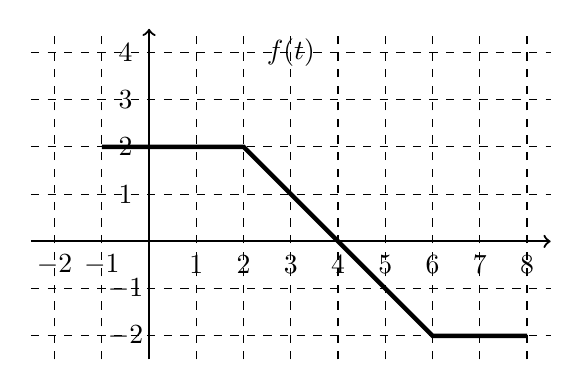
\begin{tikzpicture}[scale=.6]
\draw[thick, ->] (0,-2.5) -- (0,4.5);
\draw[thick, ->] (-2.5,0) -- (8.5,0);
\foreach \i in {-2,-1,1,2,3,4}{
	\draw[dashed] (-2.5,\i) -- (8.5,\i);
	\draw[dashed] (\i,-2.5) -- (\i,4.5);
	\node at (\i, -0.5){$\i$};
	\node at (-0.5,\i){$\i$};
	}
\foreach \i in {5,6,7,8}{
	%\draw[dashed] (-2.5,\i) -- (8.5,\i);
	\draw[dashed] (\i,-2.5) -- (\i,4.5);
	\node at (\i, -0.5){$\i$};
	%\node at (-0.5,\i){$\i$};
	}

%\draw (-.5,5) -- (0.5,5);
%\node at (-1,5.2){5};
\draw[ultra thick] (-1,2)--(2,2) -- (6,-2) -- (8,-2);
\node at (3,4){$f(t)$};
%\draw[black, line width = 0.40mm, dashed]   plot[smooth,domain=-4.2:4.2] (\x, {5-0.333*\x*\x});
\end{tikzpicture}
\end{center}

	\begin{subproblems}
	\item Determine $G(4).$
	\vspace{1in}
	\item Does $G(x)$ have a maximum on the interval $[0,8]$? Explain your answer.
	\vfill
	\end{subproblems}

%FTC part 1
\problem{6} Use the Fundamental Theorem of Calculus (Part 1) to find each derivative.
	\begin{subproblems}
	\item $\displaystyle \frac{d}{dx} \left( \int_1^x \ln(t) \: dt \right)$
	\vfill
	\item $\displaystyle \frac{d}{dx} \left( \int_{\cos(x)}^1 \sqrt{1-t^2} \: dt \right)$
	\vfill
	\end{subproblems}
\newpage
%FTC part 2
\problem{8} Evaluate each definite integral using the Fundamental Theorem of Calculus Part 2.
	\begin{subproblems}
	\item $\displaystyle \int_1^{25} \frac{2}{\sqrt{x}} \: dx$
	\vfill
	\item $\displaystyle \int_{0}^{\pi/2} (5-3\sin(x)) \: dx$
	\vfill
	\end{subproblems}

%net change
\problem{7} A ball is thrown upward from an initial height of $2 \: m$ at an initial speed of $20 \: m/s.$ Acceleration resulting from gravity is $-9.8 \: m/s^2.$ (Just to be clear, we are assuming $\:a(t)=-9.8\:$ is the equation modeling the acceleration of the ball.)\\
	\begin{subproblems}
	\item Solve for $v(t)$, the velocity of the ball $t$ seconds after it is thrown into the air.\\
	\vfill 
	\item Solve for $h(t)$, the height of the ball $t$ seconds after it is thrown into the air.\\
	\vfill 
	\end{subproblems} 
	

\end{document}
